\documentclass[10pt,twocolumn,letterpaper]{article}

\usepackage{cvpr}
\usepackage{times}
\usepackage{epsfig}
\usepackage{graphicx}
\usepackage{amsmath}
\usepackage{microtype}
\usepackage{amssymb}




% Include other packages here, before hyperref.

% If you comment hyperref and then uncomment it, you should delete
% egpaper.aux before re-running latex.  (Or just hit 'q' on the first latex
% run, let it finish, and you should be clear).
\usepackage[breaklinks=true,bookmarks=false]{hyperref}

\cvprfinalcopy % *** Uncomment this line for the final submission

\def\cvprPaperID{****} % *** Enter the CVPR Paper ID here
\def\httilde{\mbox{\tt\raisebox{-.5ex}{\symbol{126}}}}

% Pages are numbered in submission mode, and unnumbered in camera-ready
% \ifcvprfinal\pagestyle{empty}\fi
\setcounter{page}{1}
\begin{document}

%%%%%%%%% TITLE
\title{DinoQR: Time-Secured, Realtime QR Codes}

\author{
Ben Gershuny, Isaac Hilton-VanOsdall, Oscar Newman\\
Brown University\\
{\tt\small \{benjamin\_gershuny,isaac\_hilton-vanosdall,oscar\_newman\}@brown.edu}
% For a paper whose authors are all at the same institution,
% omit the following lines up until the closing ``}''.
% Additional authors and addresses can be added with ``\and'',
% just like the second author.
% To save space, use either the email address or home page, not both
}

\maketitle
%\thispagestyle{empty}

%%%%%%%%% ABSTRACT
\begin{abstract}
   We sought to apply the existing an near-universally available technology of QR codes to more secure use-cases requiring the verification of location, identify, or time. We developed a protocol for real-time animated QR code generation, scanning, and verification to provide these qualities. With the hope of expanding the technology past strict QR codes, we implemented a custom QR encoding, decoding, and scanning pipeline in Python and OpenCV2. This was functional but slow due to the limitations of Python. We also built a live server, client, and scanner demo using existing QR Code libraries as a proof of concept of the protocol. Current results are promising and we hope to combine both efforts by rewriting our QR pipeline in a low-level language.
\end{abstract}

%%%%%%%%% BODY TEXT
\section{Introduction}
Countless daily actions require verifying time, identity, or location. And many organizations, businesses, and services rely on that ability. Unfortunately, solving that problem typically requires specialized hardware (like ID cards, NFC, RFID, etc.) and software. While this is fine in certain settings, there are many that would benefit from a universally available approach. For example, venues could eliminate price-gouging secondhand markets for tickets by tying ticketing to identity and preventing transfers outside of their system. Likewise, a technology like this could be used to verify that home healthcare providers for the elderly visit their pateients when they say they do, and prevent fraud (this type of verification is now a legal requirement healthcare providers are struggling to meet). It could even be used to securely exchange secrets with trusted but potentially numerous third parties.

QR codes are a promising solution to this problem. They are universally avaialble. They can be both generated and scanned by anyone with a camera-enabled smartphone. Using modern web technology, there may not even be a need for users to download an app to scan and generate QR codes.

Unfortunately, QR codes as they exist are insecure for these applications. They can be copied, shared, replicated, and scanned by anyone at any time. They simply act as a static identifier or a shorthand for typing in some sort of code.

\subsection{Problem Statement}
In this work, we seek to create a secure, universally available, and flexible QR code pipline and protocol to provide the verificaiton of location, identity, and time to the scanner. We will achieve this through a custom encoding protocol which provides security using timestamps and cryptographic one-time passwords alongside an animated QR code displayed on a client, and a scanner and server capable of verifying those animated codes in realtime.

\section{Related Work}

Some research has focused on encoding high-density data in colored (rather than black-and-white) QR codes \cite{yang_robust_2018}. This research sought to create extremely robust high capacity QR codes using large amounts of data and multi-color-channel encoding. It identified both novel types of color interference and the best methods to avoid them.

A live event ticketing startup based in Amsterdam uses a similar approach of animating QR codes to disalow ticket resale outside of their closed system (We actually discovered them while researching this idea a few monthsa go) \cite{noauthor_guts_nodate}. They seem to have developed a robust, proprietary system for ticketing specifically, though it's not clear what additional levels of security and identify verification their protocol provides.

Ivan Daniluk, a developer from Spain, developed a system of transmitting large packets of data via quickly animating QR codes \cite{daniluk_animated_2018}. His work on this project, and later adaption of the system to error-resistent Fountail Codes provides a great model for making QR codes not only spatially but temporally robust \cite{daniluk_fountain_2018}.

\section{Methods}

\subsection{The Protocol}

\begin{figure}[t]
   \begin{center}
      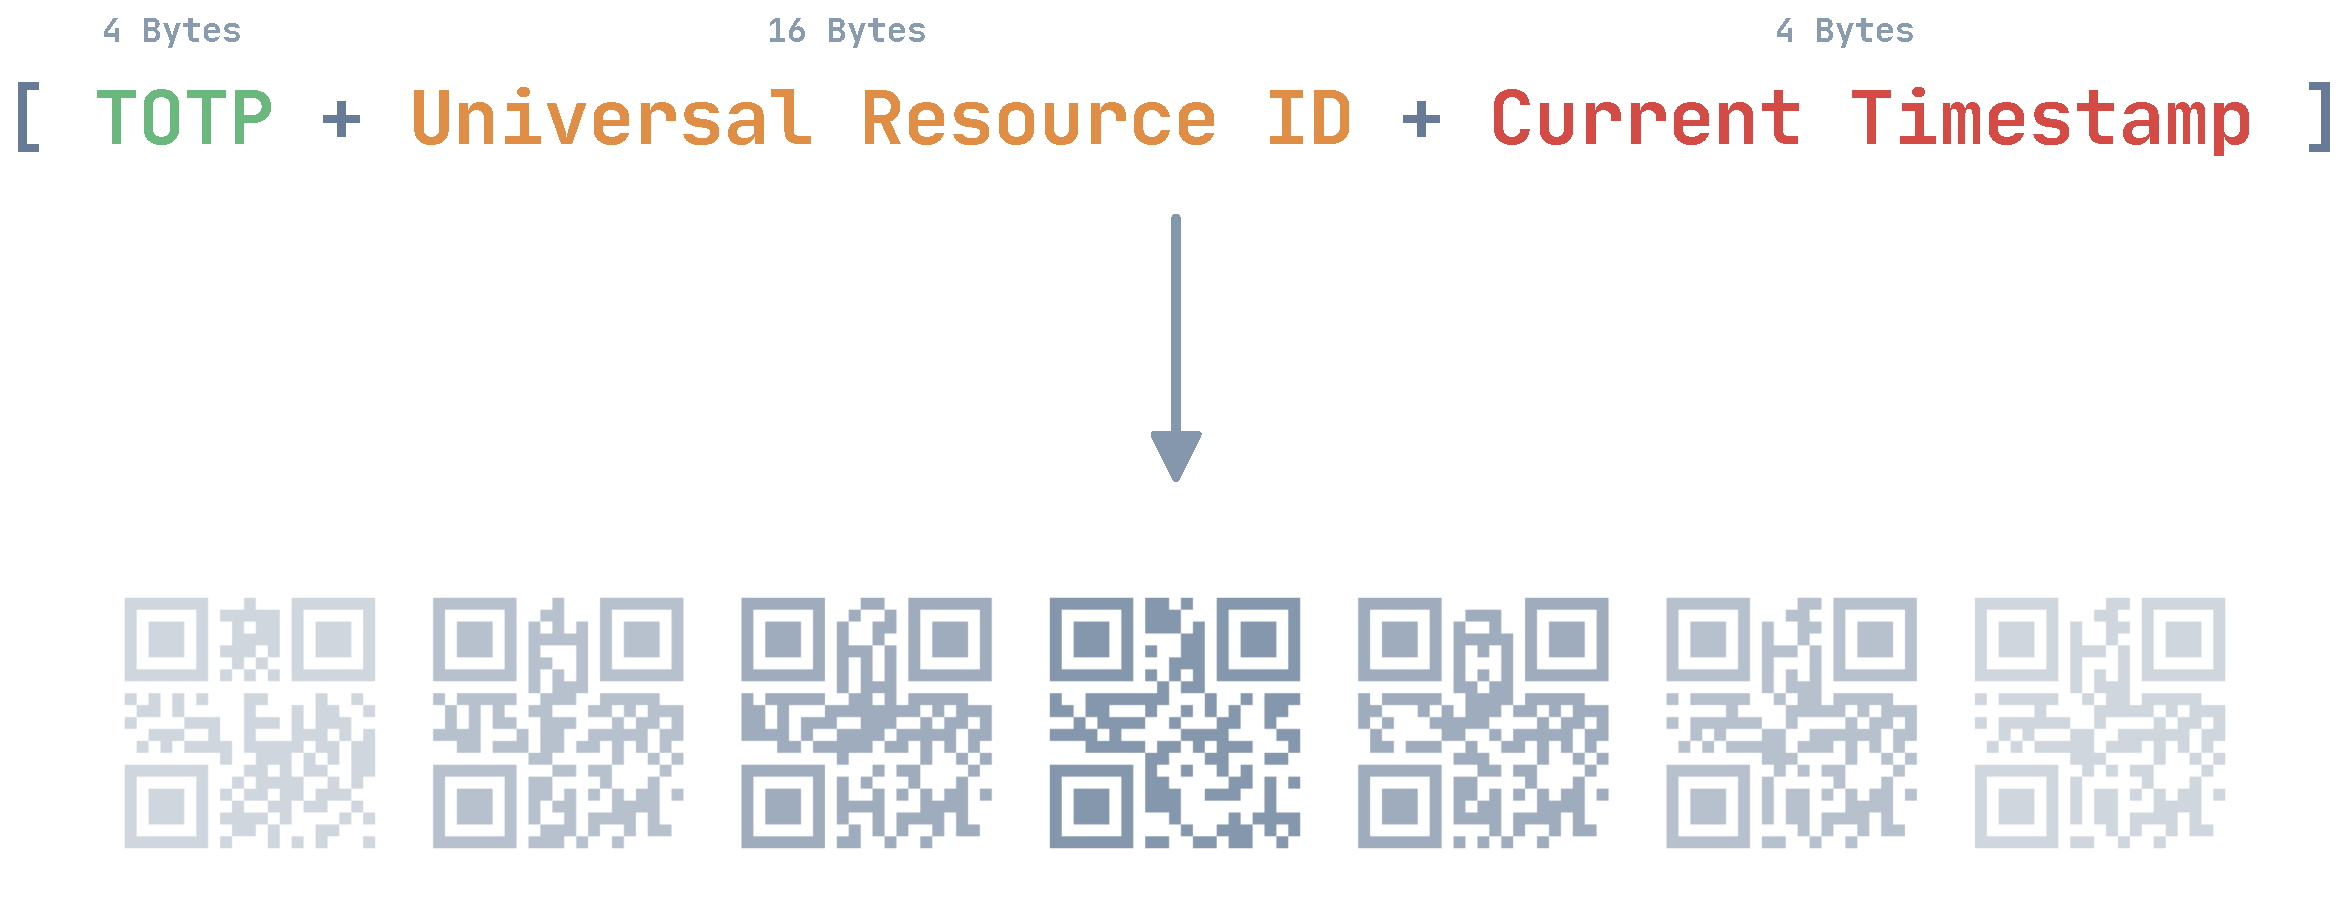
\includegraphics[width=\linewidth]{protoc.eps}
   \end{center}
      \caption{The basic layout of the protcol. TOTP and timestamp are variable with time, while Resource ID is static.}
   \label{fig:protocol}
   \end{figure}

The protocol we designed encodes, every 10th of a second, three pieces of data totaling 24 bytes into a QR code, seen in Figure \ref{fig:protocol}. Each piece of data is concatenated for into one long integer to be encoded numerically in the code—the most compact encoding QR codes support. First, it encodes a universal resource ID (a 16 bit UUID). This is constant, and allows the verification server to identify a particular resource, such as a ticket or task to be completed, relevant to the applied domain. The second part is the last four bytes of the current Unix time in milliseconds. This is the most that is needed to verify codes are generated in realtime because of the third part, which is a Time-Based One-Time Password (TOTP).\footnote{\href{https://en.wikipedia.org/wiki/Time-based_One-time_Password_algorithm}{An algorithm} which provides a unique six-digit code every 30 seconds based on a shared initial secret between a client and server}.

In this protocol, the Resource ID provides a similar function to any existing QR Code—identifying a resource that is being scanned and taking some action based upon its state. We use a universally unique UUID here such that a centeralized service could respond to a wide variety of disparate use-cases and client requests.

The current timestamp in milliseconds provides a guarantee that the code being scanned is being generated in realtime. This means that codes cannot be shared, printed, screenshotted, or even recorded for later use.

Finally, the one time password verifies client identity. A device generating a QR Code will securely store a unique salt for the TOTP shared only with the server. This means that even if someone knew a resource ID and the QR generation protocol, without the client's salt they could not recreate a valid code.

\subsection{Encoding \& Decoding}

\subsection{Detection}

Our scanning and detection step runs on Python and OpenCV bindings. It is a relatively naive scanner compared to those found in modern smartphones, but effective for our use cases (except for its speed). It first adaptively thresholds the image, assigning each pixel to either a 1-bit black or white value, based on average and local brightnesses of the image. As opposed to traditional thresholding where you specificy a specific cutoff, this is far more robust in different lighting conditions.

Next, the detector iterates through the image searching for the characteristic "finder" patterns on a QR code (the large concentric squares at the top and left-most outer corners). These patterns exhibit a consistent black:white ratio of 1:1:3:1:1, no matter what direction they are scanned from. Given this, the detector iterates through each horizontal row and identifies possible finder patterns. For each pattern it identifies, it iteratively re-checks the horizontal and vertical axes for the same ratio pattern while re-calculating the likely center of the pattern. 

Once three patterns are identified, it estimates the fourth corner and builds a bounding box. It then uses an OpenCV warp transform to crop the image exactly to the QR Code itself, represented as a bit-matrix and ready to be passed to the decoder.

The major limitation of our current implementation is speed. It takes roughly a second to process a 720p frame on a modern 8-core laptop processer. It also currently only works for upright QR Codes.

\subsection{Client and Server}

Becuase a Python-based scanning and decoding pipelien was far too slow for the realtime application our protocol required, we built a separate proof-of-concept generator, backend validation server, and mock scanner in Javascript. The frontend, including the generator and mock scanner were built in Svelte, a reactive frontent library in Javascript, using exising NodeJS QR Code generation libraries. The backend server was built using NestJS, and encoded with a fixed set of resources to respond to after verifying the codes it was sent.


\section{Results}

\subsection{QR Generation and Scanning}

\textit{Ben and Isaac, add details about decoding and encoding stuff, what works, what doesn't, is it fast or slow, etc...}

\begin{figure}[t]
   \begin{center}
      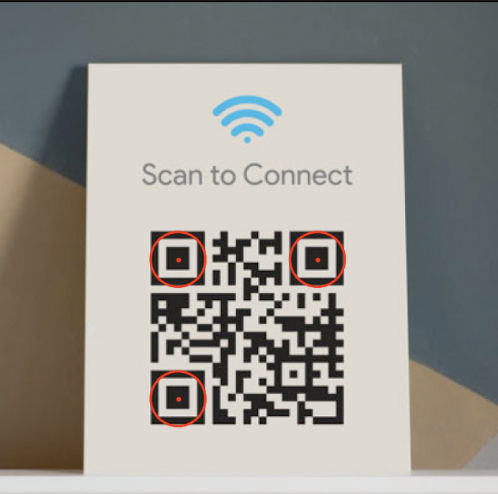
\includegraphics[width=0.8\linewidth]{print.png}
   \end{center}
      \caption{Corner detection on a printed code}
   \label{fig:print}
\end{figure}

Our scanner is promising, though not perfect. On digital images of QR Codes, like those produced by our encoder, it consistently extracts and estimates the size of the code near-perfectly, leading to a data-matrix with few errors. It even robustly identified a code's bounding box in photos of printed QR codes (Figure \ref{fig:print}).

It's failure cases are numerous, though. It struggles greatly with more distorted or specular codes, such as a 3D-printed code we used in testing. Likewise, it only works on upright orientations of codes at the moment.

Speed was the biggest flaw of the scanning pipeline, though. In our testing, the Python-based approach could scan a fame(exluding decoding), in an average of 1.6 seconds from a 720p MacBook Pro webcam. This is clearly far too slow not only for our realtime use, but too slow for most QR scanning to begin with. The source of this slowdown is largely from looping through each row and column of the image repeatedly in Python loops. A better implementation would drop into C++ for native OpenCV calls, or possibly use an alternate method of detection which is already optimized by OpenCV in Python, like contour detection.

We built a rudementary decoder to test with the scanning pipeline, and while it is fast, the complex masking and data encoding of QR codes made this part quite difficult. This decoder takes in an array of bits from the scanner and decodes the message in the QR code. We limited the scope of the decoder to QR codes with shape 21 x 21 and alphanumeric encoding. We were able to successfuly unmask the QR codes and extract the binary data from them, but we had trouble successfully decoding this stream of data that we extracted. 

\subsection{Protocol and Proof-of-Concept}

\begin{figure}[t]
   \begin{center}
      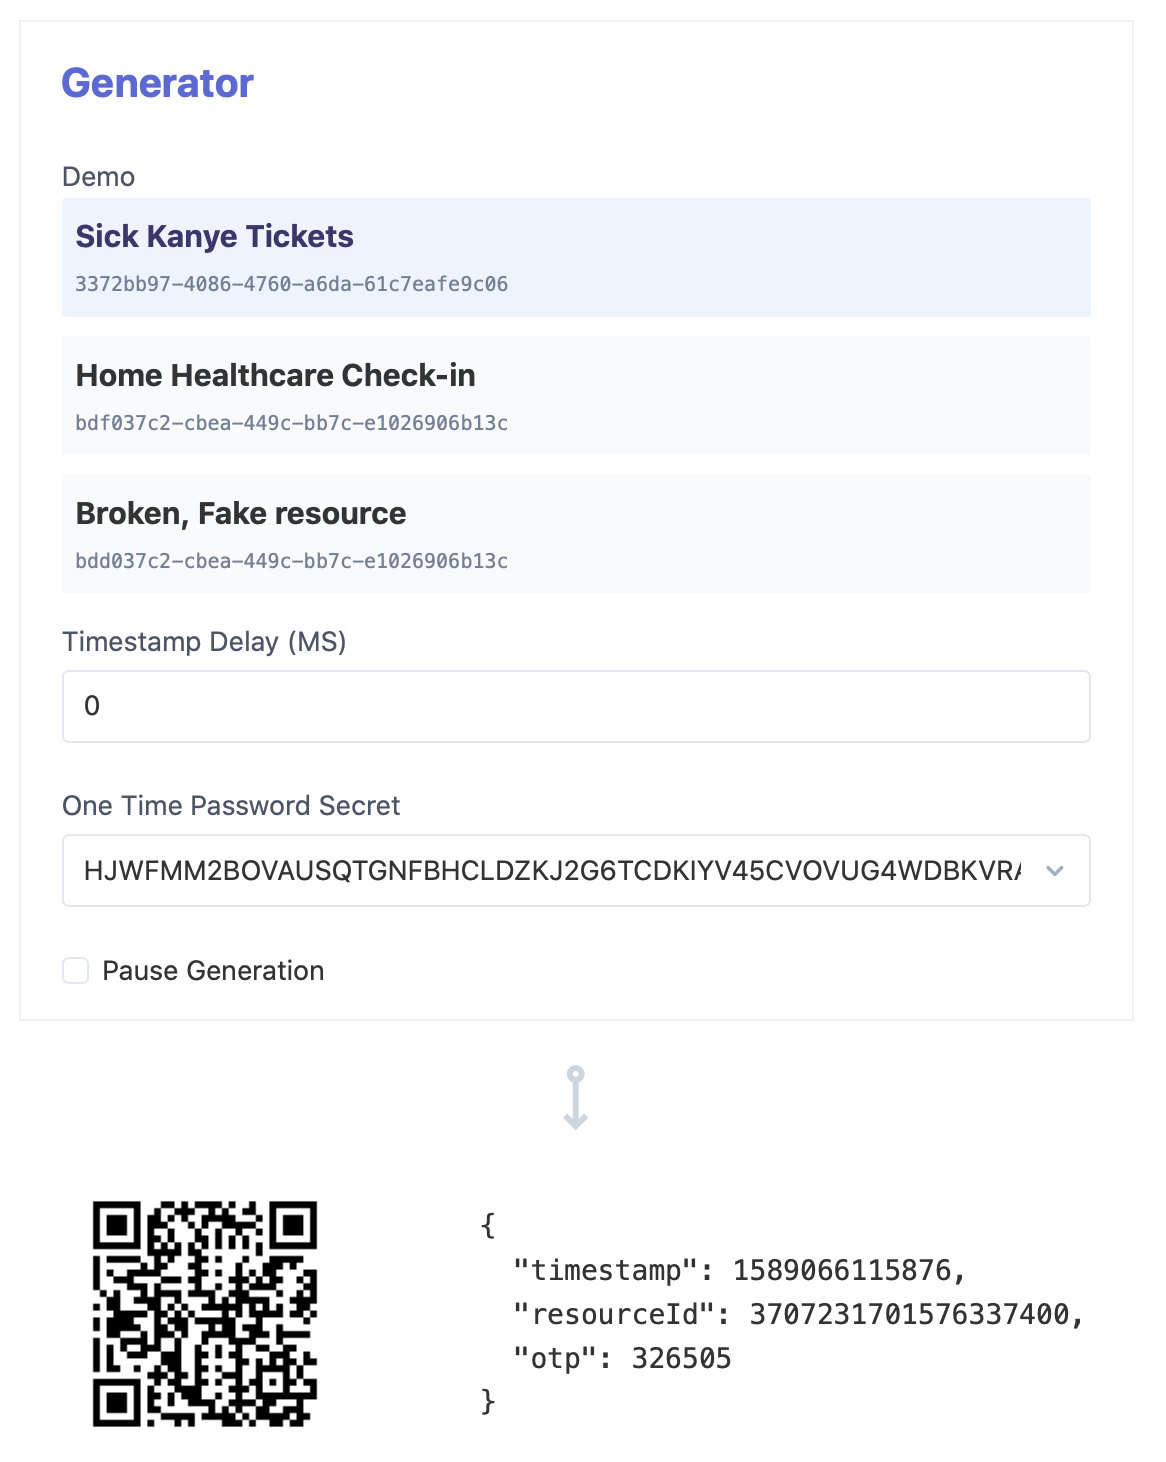
\includegraphics[width=0.8\linewidth]{gen.png}
   \end{center}
      \caption{The proof-of-concept generator.}
   \label{fig:gen}
\end{figure}


We saw great success in the mock implemenatation of our protocol. Early tests on iOS devices using native QR-reaidng frameworks were easily able to decode 10 codes per second, if not far more.

Likewise, we built the protocol into our mock client and server, deployed at \url{https://dino-demo.now.sh}, which is currently deployed live and free for anyone to test. The generator (Figure \ref{fig:gen}) and scanner (Figure \ref{fig:scan}) do not communicate other than the QR code generated, operate in realtime, and already provide robust error detection for various error cases that can be present in these codes.

Quick and easy use in a live system with an actual backend server shows great promise for the protocol and it's applicability.

\begin{figure}[t]
   \begin{center}
      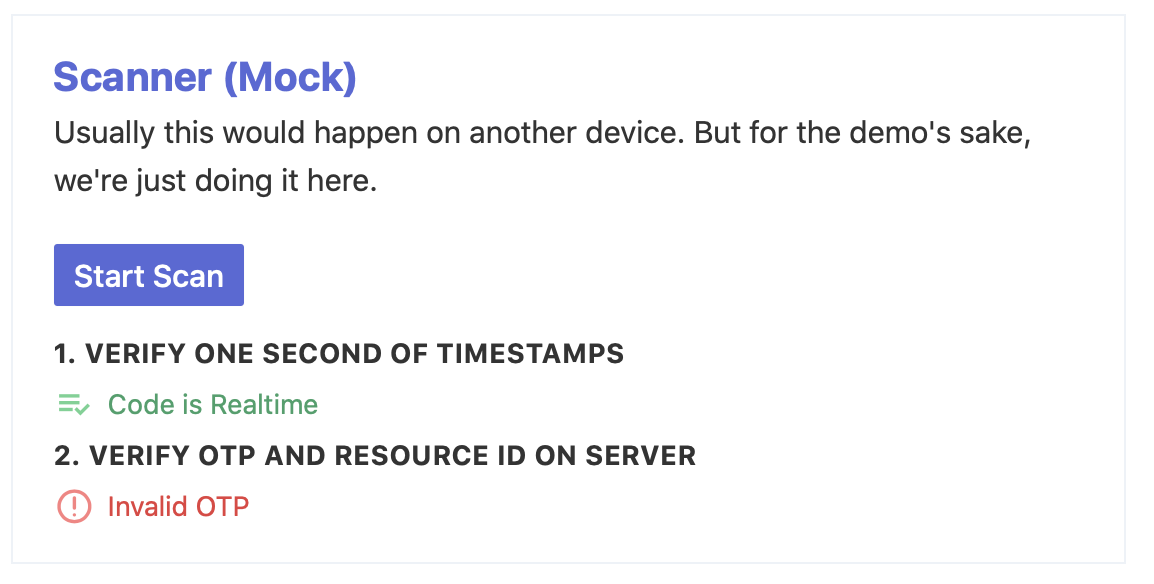
\includegraphics[width=0.8\linewidth]{scan.png}
   \end{center}
      \caption{The proof-of-concept scanner.}
   \label{fig:scan}
\end{figure}

\section{Comparaison to Existing Techniques}

As mentioned above, contour-based detection has been found to be a fast and efficient approach to detecting the bounding box of QR Codes. In this case, an edge-detection filter is typically applied to the image and a library like OpenCV detectects nested contours—some of which match the expected finder paterns. Some existing research has found massive speed improvements with optmized versions of this algorithm \cite{tong_qr_2014}. But in our testing, without serious optimization and further measures, this was an unreliable method to detect QR codes in moving images. Static images seemed to work fine, but the contour-based code was unable to consistently identify a QR code frame-to-frame, even though it ran in near-realtime.



{\small
\bibliographystyle{ieee_fullname}
\bibliography{dino}
}

\end{document}
